\documentclass[a4paper, 11pt]{article}

% -- Coments
\usepackage{verbatim}

% ----- Fonts -----
% -- Fuente --
% \usepackage{fontspec}
% \setmonofont{JetBrainsMono Nerd Font}  

% -- Color --
\usepackage{xcolor}
%\definecolor{azul}{RGB}{00,33,99}
\definecolor{azul}{RGB}{35,72,180}

% -- Page Margin --
\usepackage[margin=1in]{geometry}

% -- Espaciados --
\newcommand{\Pspace}{0.5cm}
\newcommand{\Aspace}{0.2cm}

% -- Columnas --
\usepackage{multicol}

% -- Imagenes --
\usepackage{graphicx}
\usepackage{float}

% -- Matemáticas --
\usepackage{amsmath, amssymb}

% -- Gráficas --
\usepackage{pgfplots}
\pgfplotsset{compat=1.18}


\begin{comment}
-- Formato de pregunta simple
    % - Problema n
    \vspace{\Pspace}
    \item Problema \par
        % Respuesta:
        \vspace{\Aspace} \par
        { \color{azul}  }


 -- Formato de pregunta multimple
    % - Problema 
    \vspace{\Pspace}
    \item  \par
        % Respuestas:
        \vspace{\Aspace} \par
        a) 
        \\ { \color{azul} }

        \vspace{\Aspace} \par
        b) 
        \\ { \color{azul} }


 -- Formato de imagen
\begin{figure}[!ht]
    \centering
    \includegraphics[width=0.5\textwidth]{}
\end{figure}


 -- Formato de tabla
\begin{tabular}{c|c}
    \textbf{A} & \textbf{B} \\
    \hline
    Texto & Texto \\
    Texto & Texto
\end{tabular} \\
\end{comment}


\title
{
    Fluidos y fenómenos térmicos 2026-1 \\
    Ejercicios Parcial 2
}

    \begin{document}

    \maketitle

    \begin{center}
        \begin{tabular}{r|l}
            \textbf{Expediente} & \textbf{Nombre} \\ \hline
            219208106 & Bórquez Guerrero Angel Fernando \\
        \end{tabular}
    \end{center}

    \rule{\linewidth}{0.3mm}

    {\Large \textbf{Ejercicios 24/02/2026}}
    \begin{enumerate}
    % - Problema 1
    \vspace{\Pspace}
    \item Un sistema aumenta su temperatura de 20°C a 85°C. Calcular lo siguiente: \par
        % Respuestas:
        \vspace{\Aspace} \par
        a) $\Delta T$ en °C.
        \\ { \color{azul} 
            $\Delta T = T_{f} - T_{i}$ \par
            $\Delta T = 85  \mathrm{^\circ C} - 20\mathrm{^\circ C}$ \par
            R/: $\Delta T = 65\mathrm{^\circ C}$
        }

        \vspace{\Aspace} \par
        b) $\Delta T$ en °F.
        \\ { \color{azul} 
            $20\mathrm{^\circ C} \rightarrow \frac{9}{5} (20) + 32 = 68 \mathrm{^\circ F}$ \par
            $85\mathrm{^\circ C} \rightarrow \frac{9}{5} (85) + 32 = 185\mathrm{^\circ F}$ \par
            R/: $\Delta T_{F} = 185\mathrm{^\circ F} - 68\mathrm{^\circ F} = 117\mathrm{^\circ F}$
        }

        \vspace{\Aspace} \par
        c) $\Delta T$ en K.
        \\ { \color{azul} 
            Dado que la magnitud de un grado Celsius es exactamente igual a la de un Kelvin entonces $\Delta T = 65K$
        }



    % - Problema 2
    \vspace{\Pspace}
    \item Un material se enfría de 400K a 315K. \par
        % Respuestas:
        \vspace{\Aspace} \par
        a) Calcula la diferencia en K.
        \\ { \color{azul} $\Delta K = 400K - 315K = 85K$ }

        \vspace{\Aspace} \par
        b) Calcula la diferencia en °C.
        \\ { \color{azul} $\Delta \mathrm{^\circ C} = 85\mathrm{^\circ F} $ }



    % - Problema 3
    \vspace{\Pspace}
    \item Convierte 25°C a K.\par
        % Respuesta:
        \vspace{\Aspace} \par
        { \color{azul} 25°C = 25 + 273.15 = 298.15K }



    % - Problema 4
    \vspace{\Pspace}
    \item Convierte 310K a °C. \par
        % Respuesta:
        \vspace{\Aspace} \par
        { \color{azul}  310K = 310 - 273.15 = 36.85°C}



    % - Problema 5
    \vspace{\Pspace}
    \item Convierte 77°F a °C. \par
        % Respuesta:
        \vspace{\Aspace} \par
        { \color{azul} 77°F = $(77 - 32) \times 5/9 = 25 \mathrm{^\circ C}$ }



    % - Problema 6
    \vspace{\Pspace}
    \item Convierte -40°C a °F. \par
        % Respuesta:
        \vspace{\Aspace} \par
        { \color{azul} -40 $\mathrm{^\circ C} = \frac{9}{5} (-40) + 32 = -40 \mathrm{^\circ F}$}



    % - Problema 7
    \vspace{\Pspace}
    \item Convierte 450K a °F. \par
        % Respuesta:
        \vspace{\Aspace} \par
        { \color{azul} 450K = $\mathrm{^\circ C} = \frac{9}{5} (450 - 273.15) + 32 = 350.33 \mathrm{^\circ F}$ }



    % - Problema 8
    \vspace{\Pspace}
    \item Convierte -10°F a K. \par
        % Respuesta:
        \vspace{\Aspace} \par
        { \color{azul} -10°F = $(-10 - 32) \times 5/9 + 273.14 = 249.82$K }
    \end{enumerate}


    \newpage
    {\Large \textbf{Ejercicios 02/03/2026}}
    \begin{enumerate}
    % - Problema 1
    \vspace{\Pspace}
    \item Una pista de cobre en una placa electrónica mide 8cm a 20°C. Durante operación intensa, la temperatura alcanza 85°C. Calcula cuánto se alarga la pista si $\alpha_{\text{Cu}} = 1.7 \times 10^{-5}$°C$^{-1}$ \par
        % Respuesta:
        \vspace{\Aspace} \par
        { \color{azul}  
            $L_{f} - L_{i} = \alpha L_{i} (T_{f} - T_{i})$ \par
            $L_{f} = \alpha L_{i} (T_{f} - T_{i}) + L_{i}$ \par
            $L_{f} = (1.7 \times 10^{-5}\mathrm{^\circ C^{-1}})(8cm)(85\mathrm{^\circ C} - 20\mathrm{^\circ C}) + 8cm$ \par
            $L_{f} = 8.00884cm$ \par
            R/: 0.00884cm
        }



    % - Problema 2
    \vspace{\Pspace}
    \item Un cable de fibra con refuerzo metálico mide 25m a 10°C. En verano alcanza 50°C \par
        % Respuestas:
        \vspace{\Aspace} \par
        a) ¿Cuánto se alarga con $\alpha = 1.5 \times 10^{-5}\mathrm{^\circ C^{-1}}$?
        \\ { \color{azul} 
            $L_{f} = (1.5 \times 10^{-5}\mathrm{^\circ C^{-1}})(25m)(50\mathrm{^\circ C} - 10\mathrm{^\circ C}) + 25m$ \par
            $L_{f} = 25.015m$ \par
            R/: 0.015m
        }

        \vspace{\Aspace} \par
        b) ¿Cuál es la longitud final?
        \\ { \color{azul} 
            R/: $L_{f} = 25.015m$
        }



    % - Problema 3
    \vspace{\Pspace}
    \item Una batería tiene un volumen de 0.0008$m^{3}$ a 25°C. Durante operación intensa aumenta a 40°C \par
        % Respuestas:
        \vspace{\Aspace} \par
        a) Calcula el aumento de volumen con $\beta = 6 \times 10^{-5}\mathrm{^\circ C^{-1}}$.
        \\ { \color{azul} 
            $V_{f} - V_{i} = \beta V_{i} (T_{f} - T_{i})$ \par
            $V_{f} = \beta V_{i} (T_{f} - T_{i}) + V_{i}$ \par
            $V_{f} = (6 \times 10^{-5}\mathrm{^\circ C^{-1}})(0.0008m^{3})(40 \mathrm{^\circ C} - 25 \mathrm{^\circ C}) + 0.0008m^{3}$ \par
            $V_{f} = 0.00080072m^{3}$ \par
            R/: $0.00000072m^3$
        }

        \vspace{\Aspace} \par
        b) ¿Por qué puede ser peligroso si se calienta más?
        \\ { \color{azul} 
            Al aumentar la temperatura también aumenta la presión, lo que podría hacer que la batería se incendie o hasta explote.
        }



    % - Problema 4
    \vspace{\Pspace}
    \item Un depósito contiene 3L de refrigerante a 20°C. La temperatura aumenta a 50°C \par
        % Respuestas:
        \vspace{\Aspace} \par
        a) ¿Cuál es el volumen a los 50°C con $\beta = 4 \times 10^{-4}\mathrm{^\circ C^{-1}}$?
        \\ { \color{azul} 
            $V_{f} = (4 \times 10^{-4}\mathrm{^\circ C^{-1}})(3L)(50 \mathrm{^\circ C} - 20 \mathrm{^\circ C^{-1}}) + 3L$ \par
            R/: $V_{f} = 3.036L$
        }

        \vspace{\Aspace} \par
        b) Es necesario espacio extra? ¿Por qué?
        \\ { \color{azul} 
            Sí, porque al aumentar la temperatura el refrigerante se expande y, sin espacio extra, el volumen adicional se convierte en presión que puede dañar o romper el sistema.
        }
    \end{enumerate}



    \newpage
    {\Large \textbf{Ejercicios 04/03/2026}}
    \begin{enumerate}
    % - Problema 1
    \vspace{\Pspace}
    \item La llanta de un automóvil se infla con aire a T = 10°C y presión $atm$ normal. Durante el proceso el aire se comprime 28\% de su volumen original y la temperatura aumenta 40°C \par
        % Respuestas:
        \vspace{\Aspace} \par
        a) ¿Cuál es la presión de la llanta con?
        \\ { \color{azul} 
            \textbf{Datos} \\
            $T_{i} = 10\mathrm{^\circ C}$, $T_{f} = 50\mathrm{^\circ C}$, $V_{f} = 72\%V_{i}$, $P_{i} = 1 atm$ \par

            \textbf{Fórmula} \\
            $\dfrac{P_{i} V_{i}}{T_{i}} = \dfrac{P_{f} V_{f}}{T_{if}} \rightarrow \dfrac{P_{i} V_{i} T_{f}}{T_{i}} = P_{f} V_{f} \rightarrow \dfrac{P_{i} V_{i} T_{f}}{T_{i} V_{f}} = P_{f}$ \par

            \textbf{Solución} \\
            $\dfrac{(1 atm) \times V_{i} \times (50\mathrm{^\circ C})}{(10\mathrm{^\circ C}) \times (0.72 V_{i})} = 6.94 atm$
        }

        \vspace{\Aspace} \par
        b) Después de conducir, la temperatura sube a 85°C y el volumen aumenta en 2\%. ¿Cuál es la nueva presión?
        \\ { \color{azul} 
            \textbf{Datos} \\
            $T_{i} = 50\mathrm{^\circ C}$, $T_{f} = 85\mathrm{^\circ C}$, $V_{f} = 102\%V_{i}$, $P_{i} = 6.94 atm$ \par

            \textbf{Fórmula} \\
            $\dfrac{P_{i} V_{i} T_{f}}{T_{i} V_{f}} = P_{f}$ \par

            \textbf{Solución} \\
            $\dfrac{(6.94 atm) \times V_{i} \times (85\mathrm{^\circ C})}{(50\mathrm{^\circ C}) \times (1.02 V_{i})} = 11.57 atm$
        }



    % - Problema 2
    \vspace{\Pspace}
    \item Un recipiente de 8L contiene un gas a T = 20°C y P = 9$atm$. \par
        % Respuestas:
        \vspace{\Aspace} \par
        a) Determine el número de moles.
        \\ { \color{azul} 
            \textbf{Datos} \\
            $V = 8L$, $T = 20$°C, $P = 9 atm$, $R = 8.314 \frac{J}{mol * K}$ \\
            $V = 0.008 m^{3}$ \\
            $T = 293.15 K$ \\
            $P = 911925 Pa$ \par

            \textbf{Fórmula} \\
            $PV = nRT \rightarrow \dfrac{PV}{RT} = n$ \par

            \textbf{Solución} \\
            $\dfrac{(911925 Pa)(0.008 m^{3})}{(8.314 J/(mol * K))(293.15 K)} = 2.993 mol$
        }

        \vspace{\Aspace} \par
        b) ¿Cuántas moléculas hay en el recipiente (N)?
        \\ { \color{azul} 
            $N_{A} = 6.022 \times 10^{23}mol^{-1}$ \par
            $N = (2.993) \times (6.022 \times 10^{23}mol^{-1}) = 1.802 \times 10^{24}$ moléculas.
        }
 


    % - Problema 3
    \newpage
    \item 9g de agua se ponen en una olla de presión de 2L y se calienta a 500°C. ¿Cuál es la presión dentro del contenedor? \par
        % Respuesta:
        \vspace{\Aspace} \par
        { \color{azul}  
            \textbf{Datos} \\
            $V = 0.002m^{3}$, $T = 500$°C, $m = 9g$ \\
            $T = 773.15 K$ \\
            $M_{\text{agua}} = 18.015 g/mol$ \\
            $n = \dfrac{9g}{18.015 g/mol} = 0.5 mol$ \par

            \textbf{Fórmula} \\
            $PV = nRT \rightarrow P = \dfrac{nRT}{V}$ \par

            \textbf{Solución} \\
            $P = \dfrac{(0.5 mol)(8.314 J/(mol * K))(773.15 K)}{0.002 m^{3}} = 1,606,992.275 Pa$
        }



    % - Problema 4
    \vspace{\Pspace}
    \item 25m bajo la superficie del mar ($\rho = 1025 kg/m^3$), donde $T = 5$°C un buso exhala una burbuja de aire con $V = 1cm^3$. Si la $T$ de la superficie es de 20°C. ¿Cuál es el volumen de la burbuja justo antes de romper en la superficie? \par
        % Respuesta:
        \vspace{\Aspace} \par
        { \color{azul}  
            \textbf{Datos} \\
            $h = 25m$, $\rho = 1025 kg/m^{3}$, $V_{i} = 1 cm^{3}$, $T_{i} = 5$°C, $T_{f} = 20$°C, $1 atm = 1.013 \times 10^{5} Pa$, $R = 8.314 J/(mol * K)$ \\
            $P_{i} = \rho g h = (1025 kg/m^{3}) (9.81 m/s^{2}) (25m) = 251,381.25 Pa$ \par

            \textbf{Fórmula} \\
            $\dfrac{P_{i} V_{i}}{T_{i}} = \dfrac{P_{f} V_{f}}{T_{f}} \rightarrow \dfrac{P_{i} V_{i} T_{f}}{T_{i} P_{f}} = V_{f}$ \par

            \textbf{Solución} \\
            $\dfrac{(251381.25 Pa + 1.013 \times 10^{5} Pa) (1 cm^{3}) (20\text{°C})}{(5\text{°C}) (1.013 \times 10^5 Pa)} = 13.92 cm^{3}$
        }
    \end{enumerate}



    \newpage
    {\Large \textbf{Ejercicios 10/03/2026}}
    \begin{enumerate}
    % - Problema 1
    \vspace{\Pspace}
    \item Considere el aparato de joule con dos masas de 1.5kg cada una, que caen de una altura de 3m, y donde el tanque está lleno de 200g de agua. ¿Cuál es el aumento de temperatura del agua al girar las aspas? \par
        % Respuesta:
        \vspace{\Aspace} \par
        { \color{azul}  
            \textbf{Datos} \\
            $m = 1.5 kg$, $m_{\text{agua}} = 200g$, $h = 3m$, $C_{\text{agua}} = 4.18 \times 10^{3} J/kg\mathrm{^\circ C}$ \\
            $m_{\text{agua}} = 0.2 kg$ \\
            $U = (1.5kg) (9.81 m/s^{2}) (3m) = 44.1 J$ \\
            $\Delta U = 2 mgh = 88.2 J$ \\
            $W = \Delta U + \Delta K \rightarrow W = \Delta U$ \par

            \textbf{Fórmula} \\
            $C = \dfrac{Q}{m \Delta T} \rightarrow C \Delta T = \dfrac{Q}{m} \rightarrow \Delta T = \dfrac{Q}{mC}$ \par

            \textbf{Solución} \\
            $\Delta T = \dfrac{88.2 J}{(0.2 kg) (4.18 \times 10^3 J/kg\mathrm{^\circ C})} = 0.1055\mathrm{^\circ C}$
        }



    % - Problema 2
    \vspace{\Pspace}
    \item La temperatura de una barra de plata se eleva 10°C cuando absorbe 1.23kJ de energía en forma de calor. La masa de la barra es de 525g. ¿Cuál es el calor específico del plomo? \par
        % Respuesta:
        \vspace{\Aspace} \par
        { \color{azul}  
            \textbf{Datos} \\
            $\Delta T = 10\mathrm{^\circ C}$, $m = 525g$, $Q = 1.23kJ$ \\
            $m = 0.525 kg$ \\
            $Q = 1230 J$ \par

            \textbf{Fórmula} \\
            $C = \dfrac{Q}{m \Delta T}$ \par

            \textbf{Solución} \\
            $C = \dfrac{1230 J}{(0.525 kg) (10\mathrm{^\circ C})} = 234.29 J/kg*\mathrm{^\circ C}$
        }



    % - Problema 3
    \vspace{\Pspace}
    \item Un bloque de aluminio de 500g se calienta desde 20°C a 80°C. Calcula la energía necesaria para lograr ese aumento de temperatura. \par
        % Respuesta:
        \vspace{\Aspace} \par
        { \color{azul}  
            \textbf{Datos} \\
            $m = 500g$, $T_{i} = 20\mathrm{^\circ C}$, $T_{f} = 80\mathrm{^\circ C}$, $C_{aluminio} = 900 J/kg\mathrm{^\circ C}$ \\
            $m = 0.5 kg$ \\
            $\Delta T = 60\mathrm{^\circ C}$ \par

            \textbf{Fórmula} \\
            $Q = C m \Delta T$

            \textbf{Solución} \\
            $Q = (900 J/kg\mathrm{^\circ C}) (0.5 kg) (60\mathrm{^\circ C}) = 27000 J$
        }



    % - Problema 4
    \newpage
    \item ¿Cuánta penergía total se requiere para convertir un cubo de 40g de hielo de -10°C a vapor a 110°C? \par
        % Respuesta:
        \vspace{\Aspace} \par
        { \color{azul} 
            \textbf{Datos} \\
            $m = 40g = 0.04kg$, $T_{i} = -10\mathrm{^\circ C}$, $T_{f} = 110\mathrm{^\circ C}$ \\
            $C_{hielo} = 2090 J/kg\cdot\mathrm{^\circ C}$, $C_{agua} = 4186 J/kg\cdot\mathrm{^\circ C}$, $C_{vapor} = 2010 J/kg\cdot\mathrm{^\circ C}$ \\
            $L_{f} = 3.33 \times 10^{5} J/kg$, $L_{v} = 2.26 \times 10^{6} J/kg$ \par

            \textbf{Fórmula} \\
            $Q_{total} = Q_{hielo} + Q_{fusion} + Q_{agua} + Q_{ebullicion} + Q_{vapor}$ \\
            $Q_{total} = m(C_{hielo}\Delta T_1 + L_f + C_{agua}\Delta T_2 + L_v + C_{vapor}\Delta T_3)$ \par

            \textbf{Solución} \\
            $Q_{total} = 0.04( (2090)(10) + 333000 + (4186)(100) + 2260000 + (2010)(10) )$ \\
            $Q_{total} = 0.04(20900 + 333000 + 418600 + 2260000 + 20100)$ \\
            $Q_{total} = 122,104 J = 122.1 kJ$
        }
    \end{enumerate}



    \newpage
    {\Large \textbf{Ejercicios 18/03/2026}}
    \begin{enumerate}
    % - Problema 1
    \vspace{\Pspace}
    \item 1g de agua se vaporiza isobáricamente a 1 atm. Su volumen en el estado líquido $V_{i} = V_{\text{líquido}} = 1cm^{3}$ y su volumen en el estado de vapor es $V_{f} = V_{\text{vapor}} = 1671cm^{3}$. Encuentre el trabajo invertido en la expansión y el cambio de energía en el sistema. No hay cambio de temperatura. \par
        % Respuesta:
        \vspace{\Aspace} \par
        { \color{azul} 
            \textbf{Datos} \\
            $m = 1g = 0.001kg$, $P = 1 atm = 101325 Pa$, $V_i = 1 \times 10^{-6} m^3$, $V_f = 1671 \times 10^{-6} m^3$ \\
            $L_v = 2.26 \times 10^6 J/kg$ \par

            \textbf{Fórmula} \\
            $W = P \Delta V = P(V_f - V_i)$ \\
            $Q = m L_v$ \\
            $\Delta E_{int} = Q - W$ \par

            \textbf{Solución} \\
            $W = (101325 Pa)(1670 \times 10^{-6} m^3) = 169.2 J$ \\
            $Q = (0.001 kg)(2.26 \times 10^6 J/kg) = 2260 J$ \\
            $\Delta E_{int} = 2260 J - 169.2 J = 2090.8 J$
        }



    % - Problema 2
    \vspace{\Pspace}
    \item Una muestra de un gas ideal pasa por el proceso que se muestra a continuación. \par
    \begin{figure}[!ht]
        \hspace{1cm}
        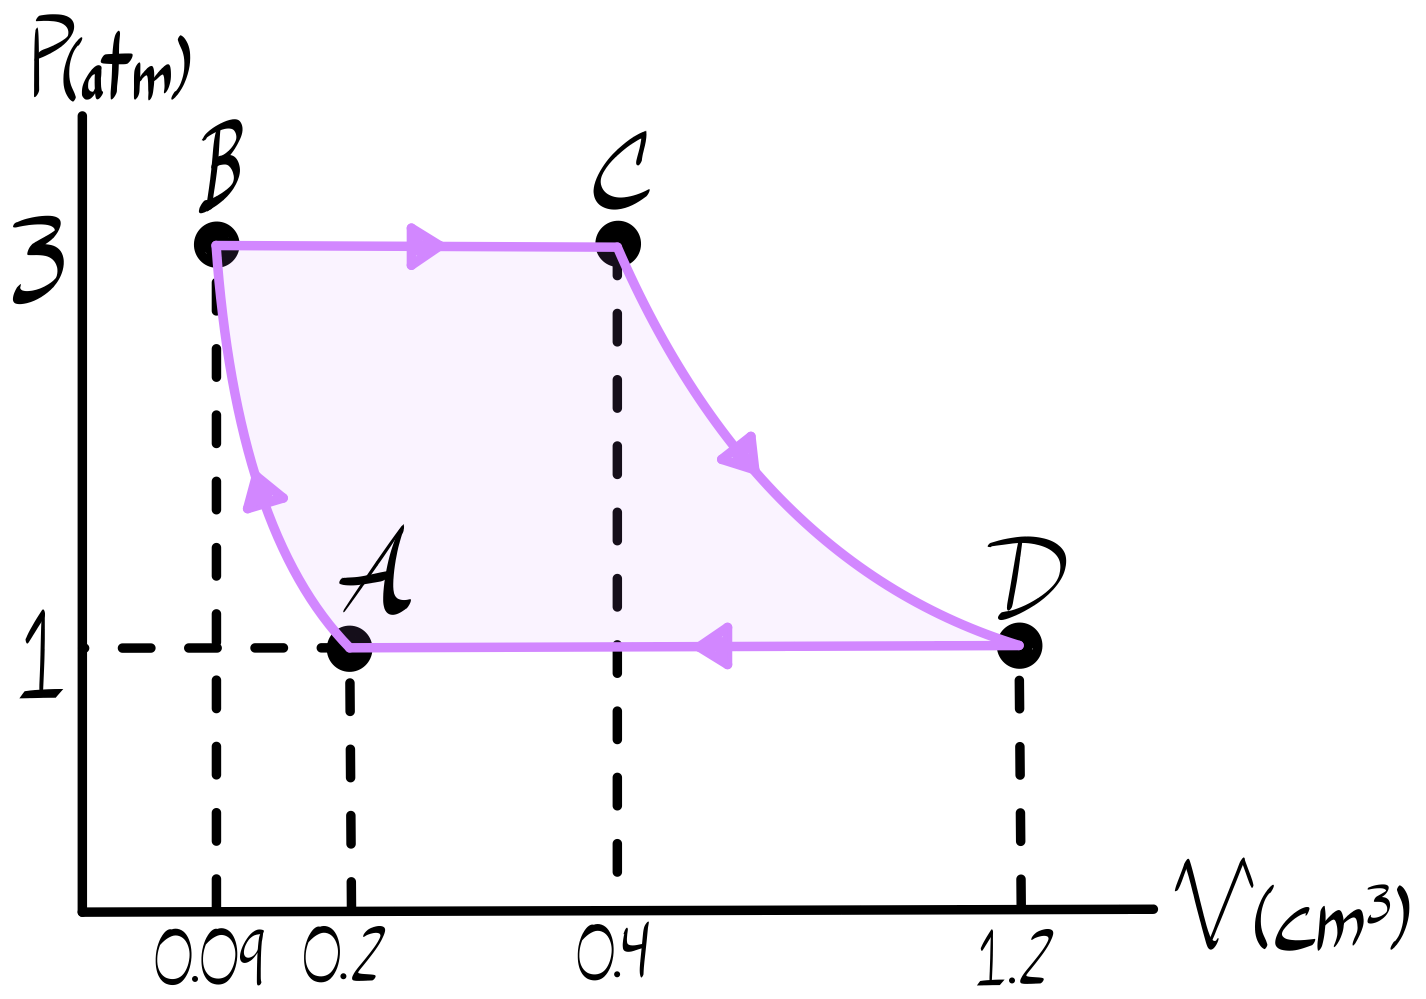
\includegraphics[width=0.45\textwidth]{./images/diagrama.jpg}
    \end{figure}
    \begin{itemize}
        \item De $A$ a $B$ el proceso es adiabático.
        \item De $B$ a $C$ el isobárico con 100kJ de energía que entran al sistema por calor.
        \item De $C$ a $D$ es isotérmico.
        \item De $D$ a $A$ es isobárico con 150kJ de energía que salen del sistema por calor.
    \end{itemize}
    Determine el cambio en la energía interna $E_{\text{int}_{B}} - E_{\text{int}_{A}}$.
        % Respuesta:
        \vspace{\Aspace} \par
        { \color{azul} 
            \textbf{Datos} \\
            $\Delta E_{Ciclo} = 0$, $Q_{BC} = 100kJ$, $Q_{DA} = -150kJ$ \par

            \textbf{Fórmula} \\
            $\Delta E_{Ciclo} = \Delta E_{AB} + \Delta E_{BC} + \Delta E_{CD} + \Delta E_{DA} = 0$ \\
            En un proceso isotérmico (C a D): $\Delta E_{CD} = 0$ \\
            En procesos isobáricos para gases ideales: $\Delta E = Q / \gamma$ \par

            \textbf{Solución} \\
            $\Delta E_{AB} + \frac{Q_{BC}}{\gamma} + 0 + \frac{Q_{DA}}{\gamma} = 0$ \\
            $\Delta E_{AB} = \frac{-(100 kJ - 150 kJ)}{\gamma} = \frac{50 kJ}{\gamma}$ \\
            $E_{\text{int}_{B}} - E_{\text{int}_{A}} = \Delta E_{AB} = \frac{50 kJ}{1.4} = 35.71 kJ$
        }



    % - Problema 3
    \vspace{\Pspace}
    \item Un mol de gas ideal realiza 3000J de trabajo sobre sus alrededores a medida que se expande isotérmicamente hasta una presión final de 1atm y 25L de volumen. \par
        % Respuestas:
        \vspace{\Aspace} \par
        a) Determine el volumen inicial.
        \\ { \color{azul} 
            \textbf{Datos} \\
            $n = 1 mol$, $W = 3000 J$, $P_f = 1 atm = 101325 Pa$, $V_f = 25L = 0.025 m^3$ \par

            \textbf{Fórmula} \\
            Para proceso isotérmico: $W = P_f V_f \ln \left( \frac{V_f}{V_i} \right) \rightarrow \ln \left( \frac{V_f}{V_i} \right) = \frac{W}{P_f V_f}$ \par

            \textbf{Solución} \\
            $\ln \left( \frac{V_f}{V_i} \right) = \frac{3000 J}{(101325 Pa)(0.025 m^3)} = 1.1843$ \\
            $\frac{V_f}{V_i} = e^{1.1843} = 3.2684 \rightarrow V_i = \frac{25L}{3.2684} = 7.649 L$
        }

        \vspace{\Aspace} \par
        b) Determine la temperatura del gas.
        \\ { \color{azul} 
            \textbf{Fórmula} \\
            $P_f V_f = nRT_f \rightarrow T_f = \frac{P_f V_f}{nR}$ \par

            \textbf{Solución} \\
            $T_f = \frac{(101325 Pa)(0.025 m^3)}{(1 mol)(8.314 J/mol \cdot K)} = 304.68 K$
        }
    \end{enumerate}



    \newpage
    {\Large \textbf{Ejercicios 20/03/2026}}
    \begin{enumerate}
    % - Problema 1
    \vspace{\Pspace}
    \item Una máquina térmica admite 360J de energía de un depósito caliente y realiza 25J de trabajo en cada ciclo. \par
        % Respuestas:
        \vspace{\Aspace} \par
        a) Encuentre la eficiencia de la máquina.
        \\ { \color{azul} 
            \textbf{Fórmula} \\
            $e = \frac{W}{Q_h}$ \par
            \textbf{Solución} \\
            $e = \frac{25 J}{360 J} = 0.0694 = 6.94\%$
        }

        \vspace{\Aspace} \par
        b) La energía expulsada en el depósito frío en cada cilo
        \\ { \color{azul} 
            \textbf{Fórmula} \\
            $W = Q_h - Q_c \rightarrow Q_c = Q_h - W$ \par
            \textbf{Solución} \\
            $Q_c = 360 J - 25 J = 335 J$
        }



    % - Problema 2
    \vspace{\Pspace}
    \item Una máquina térmica tiene una potencia de 5 kW y eficiencia del 25\%. La máquina expulsa 8kJ de energía en cada ciclo. \par
        % Respuestas:
        \vspace{\Aspace} \par
        a) Encuentre la energía que admite en cada ciclo.
        \\ { \color{azul} 
            \textbf{Fórmula} \\
            $e = 1 - \frac{Q_c}{Q_h} \rightarrow \frac{Q_c}{Q_h} = 1 - e \rightarrow Q_h = \frac{Q_c}{1 - e}$ \par
            \textbf{Solución} \\
            $Q_h = \frac{8000 J}{1 - 0.25} = 10,666.67 J = 10.66 kJ$
        }

        \vspace{\Aspace} \par
        b) Encuentre el intervalo de tiempo de cada ciclo.
        \\ { \color{azul} 
            \textbf{Fórmula} \\
            $W = Q_h - Q_c$ \\
            $Potencia = \frac{W}{t} \rightarrow t = \frac{W}{Potencia}$ \par
            \textbf{Solución} \\
            $W = 10666.67 J - 8000 J = 2666.67 J$ \\
            $t = \frac{2666.67 J}{5000 J/s} = 0.533 s$
        }



    % - Problema 3
    \vspace{\Pspace}
    \item Una máquina térmica absorbe 1200J de un foco caliente y libera 700J al foco frío. \par
        % Respuestas:
        \vspace{\Aspace} \par
        a) Calcula el trabajo realizado.
        \\ { \color{azul} 
            \textbf{Solución} \\
            $W = Q_h - Q_c = 1200 J - 700 J = 500 J$
        }

        \vspace{\Aspace} \par
        b) Calcula la eficiencia.
        \\ { \color{azul} 
            \textbf{Solución} \\
            $e = \frac{W}{Q_h} = \frac{500 J}{1200 J} = 0.4167 = 41.67\%$
        }



    % - Problema 4
    \newpage
    \item Una máquina tiene una eficiencia del 30\% y recibe 2000J de calor. \par
        % Respuestas:
        \vspace{\Aspace} \par
        a) Calcule el trabajo.
        \\ { \color{azul} 
            \textbf{Solución} \\
            $W = e \times Q_h = 0.30 \times 2000 J = 600 J$
        }

        \vspace{\Aspace} \par
        b) Calcule cuánto calor se deshecha.
        \\ { \color{azul} 
            \textbf{Solución} \\
            $Q_c = Q_h - W = 2000 J - 600 J = 1400 J$
        }
    \end{enumerate}



    \newpage
    {\Large \textbf{Ejercicios 20/03/2026}}
    \begin{enumerate}
    % - Problema 1
    \vspace{\Pspace}
    \item Una charola de hielo contiene 500g de agua líquida a 0°C. Calcule el cambio en la entropía del agua cuando se congela lenta y completamente a 0°C \par
        % Respuesta:
        \vspace{\Aspace} \par
        { \color{azul} 
            \textbf{Datos} \\
            $m = 0.5kg$, $T = 0\mathrm{^\circ C} = 273.15K$, $L_f = 3.33 \times 10^5 J/kg$ \par

            \textbf{Fórmula} \\
            $\Delta S = \frac{Q}{T}$ \\
            $Q = m L_f$ \par

            \textbf{Solución} \\
            $Q = -(0.5 kg)(3.33 \times 10^5 J/kg) = 166,500 J$ \\
            $\Delta S = \frac{-166500 J}{273.15 K} = 609.55 J/K$
        }



    % - Problema 2
    \vspace{\Pspace}
    \item Una masa de plomo de 3kg se funda a 327.3°C. Su $L_{f}$ es de $2.45x10^{4}$ J/kg. ¿Cuál es el cambio en la entropía? \par
        % Respuesta:
        \vspace{\Aspace} \par
        { \color{azul} 
            \textbf{Datos} \\
            $m = 3kg$, $T = 327.3\mathrm{^\circ C} + 273.15 = 600.45K$, $L_f = 2.45 \times 10^4 J/kg$ \par

            \textbf{Fórmula} \\
            $\Delta S = \frac{Q}{T} = \frac{m L_f}{T}$ \par

            \textbf{Solución} \\
            $\Delta S = \frac{(3 kg)(2.45 \times 10^4 J/kg)}{600.45 K} = \frac{73500 J}{600.45 K} = 122.41 J/K$
        }



    % - Problema 3
    \vspace{\Pspace}
    \item Un bloque de aluminio de 0.8kg se calienta de 20°C a 80°C. Calcula el cambio en la entropía con $C_{Al} = 900 J/kg * °C$. \par
        % Respuesta:
        \vspace{\Aspace} \par
        { \color{azul} 
            \textbf{Datos} \\
            $m = 0.8kg$, $T_i = 293.15K$, $T_f = 353.15K$, $C_{Al} = 900 J/kg \cdot K$ \par

            \textbf{Fórmula} \\
            $\Delta S = m C \ln \left( \frac{T_f}{T_i} \right)$ \par

            \textbf{Solución} \\
            $\Delta S = (0.8 kg)(900 J/kg \cdot K) \ln \left( \frac{80}{20} \right) = 998.131 J/C$
        }



    % - Problema 4
    \vspace{\Pspace}
    \item Dos sistemas reciben 1000 J de calor:
    \begin{itemize}
        \item A está a 500k.
        \item B está a 250k.
    \end{itemize}
        % Respuestas:
        \vspace{\Aspace} \par
        a) Calcula $\Delta S$ para cada uno.
        \\ { \color{azul} 
            \textbf{Solución} \\
            $\Delta S_A = \frac{1000 J}{500 K} = 2 J/K$ \\
            $\Delta S_B = \frac{1000 J}{250 K} = 4 J/K$
        }

        \vspace{\Aspace} \par
        b) ¿En cuál aumenta más la entropía y por qué?
        \\ { \color{azul} 
            Cuando introduces la misma cantidad de calor (1000 J) en un sistema más frío (250 K), estás causando un ``desorden" relativo mucho mayor que si lo introduces en un sistema que ya estaba muy caliente y agitado (500 K).
        }
    \end{enumerate}
\end{document}
